Una empresa de distribución (LogiMax S.A.) quiere conectar sus centros de distribución en distintas ciudades minimizando el coste total de infraestructura de fibra óptica. Cada conexión entre ciudades tiene un coste asociado (en miles de \euro). La empresa quiere construir una red que conecte todos los centros minimizando el coste total. Aplicando y explicando los métodos estudiados en la asignatura, ¿qué red debe construir y qué coste tiene?

\begin{center}
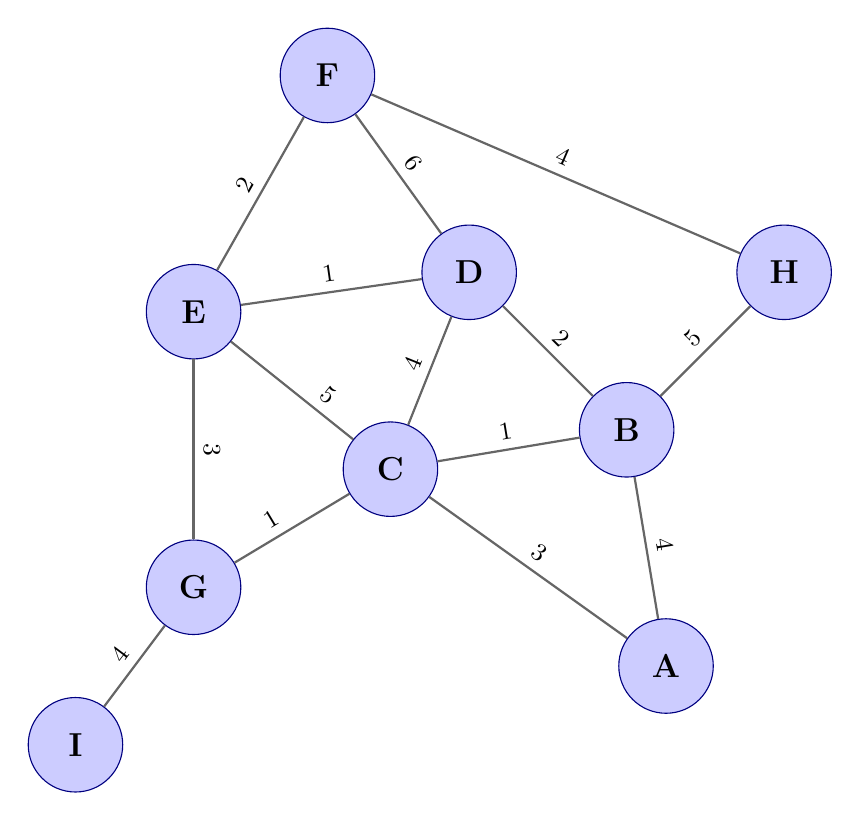
\begin{tikzpicture}
    % Estilo para los nodos
    \tikzstyle{node_style} = [circle, draw=blue!50!black, fill=blue!20, minimum size=1.2cm, font=\large\bfseries]

    % Estilo para las aristas
    \tikzstyle{edge_style} = [-, thick, draw=gray!80!black]
    
    % Estilo para las etiquetas de las aristas
    \tikzstyle{label_style} = [sloped, midway, auto, font=\small]

    % Definición de los nodos con sus posiciones aproximadas
    \node[node_style] (A) at (7, 0.5) {A};
    \node[node_style] (B) at (6.5, 3.5) {B};
    \node[node_style] (C) at (3.5, 3) {C};
    \node[node_style] (D) at (4.5, 5.5) {D};
    \node[node_style] (E) at (1, 5) {E};
    \node[node_style] (F) at (2.7, 8) {F};
    \node[node_style] (G) at (1, 1.5) {G};
    \node[node_style] (H) at (8.5, 5.5) {H};
    \node[node_style] (I) at (-0.5, -0.5) {I};

    % Conexiones y pesos de las aristas (basado en el archivo grafo_final_A_I.png)
    \draw[edge_style] (A) to node[label_style, pos=0.5] {4} (B);
    \draw[edge_style] (A) to node[label_style, pos=0.5] {3} (C);
    
    \draw[edge_style] (B) to node[label_style, pos=0.5] {2} (D);
    \draw[edge_style] (B) to node[label_style, pos=0.5] {1} (C);
    \draw[edge_style] (B) to node[label_style, pos=0.5] {5} (H);
    
    \draw[edge_style] (C) to node[label_style, pos=0.3] {5} (E);
    \draw[edge_style] (C) to node[label_style, pos=0.6] {1} (G);
    %\draw[edge_style] (C) to node[label_style, pos=0.6] {6} (G); % Nota: Dos aristas G-C
    
    \draw[edge_style] (D) to node[label_style, pos=0.5] {6} (F);
    \draw[edge_style] (D) to node[label_style, pos=0.5] {1} (E);
    \draw[edge_style] (D) to node[label_style, pos=0.5] {4} (C); % Corregido: D-C, no D-H
    
    \draw[edge_style] (E) to node[label_style, pos=0.5] {2} (F);
    \draw[edge_style] (E) to node[label_style, pos=0.5] {3} (G);
    
    \draw[edge_style] (F) to node[label_style, pos=0.5] {4} (H);
    
   % \draw[edge_style] (G) to node[label_style, pos=0.5] {2} (H);
    \draw[edge_style] (G) to node[label_style, pos=0.5] {4} (I);
   % \draw[edge_style] (G) to node[label_style, pos=0.5] {1} (C); % Nota: Dos aristas G-C
    %\draw[edge_style] (G) to node[label_style, pos=0.5] {6} (C); % Nota: Dos aristas G-C

\end{tikzpicture}
\end{center}